% Created 2024-10-16 śro 21:35
% Intended LaTeX compiler: pdflatex
\documentclass[../../main.tex]{subfiles}

% \usepackage[a4paper, margin=3cm]{geometry}
% \usepackage{amssymb} // not working

\usepackage[T1]{fontenc}
\usepackage[utf8]{inputenc}
\usepackage{graphicx}
\usepackage{longtable}
\usepackage{wrapfig}
\usepackage{rotating}
\usepackage[normalem]{ulem}
\usepackage{amsmath}
\usepackage{capt-of}
\usepackage{hyperref}
\usepackage{siunitx}
\usepackage{float}
\usepackage[polish]{babel}

\graphicspath{{../}}
\author{Wojciech Paderewski}
\date{\today}
\title{Koncepcja ukladu}
\hypersetup{
 pdfauthor={Wojciech Paderewski},
 pdftitle={Koncepcja ukladu},
 pdfkeywords={},
 pdfsubject={},
 pdflang={Polish}}
 
\begin{document}

\subsection{Przetwornica 12V na HV}
\subsubsection{Wybór układu scalonego}
Wybrano układ LM3488 produkcji Texas Instruments, który jest układem przeznaczonym do budowy przetwornic typu Boost oraz Flyback. 
Jest to układ high efficiency, co jest powodem dla którego został wybrany.

\subsubsection{Założenia projektowe}
\begin{itemize}
    \item Napięcie wejściowe: 12\si{\volt}
    \item Napięcie wyjściowe: 130-220\si{\volt}
    \item Prąd wyjściowy: 20\si{\milli\ampere}
    \item 0.1\si{\volt} tętnienia napięcia wyjściowego
    \item Częstotliwość przełączania: 400\si{\kilo\hertz}
\end{itemize}

Jako początkowe założenie przyjęto częstotliwość przełączania 400kHz zgodnie z domyślną wartością w nocie katalogowej układu, 
ale możliwe jest zwiększanie częstotliwości do 1MHz, co pozwala na zmniejszenie rozmiarów cewki oraz kondensatorów, natomiast może to
pogorszyć sprawność układu, ponieważ według noty katalogowej wraz ze wzrostem częstotliwości spada wzmocnienie układu, co przekłada się na mniejszą sprawność.

\subsubsection{Dobór cewki}
Oszacowano wartość prądu cewki na podstawie założonego prądu wyjściowego:

\begin{equation}
    I_{l} = \frac{V_{out} \cdot I_{out}}{V_{in}} = \frac{220 \cdot 0.02}{12} \approx 0.36\si{\ampere}
\end{equation}

Dodatkowe 30\% prądu wyjściowego zostało dodane jako tętnienia prądu, co pozwala oszacować wartość maksymalnego prądu cewki:
\begin{equation}
    I_{peak} = (1+0.3) \cdot I_{l} = 1.3 \cdot 0.36 \approx 0.468\si{\ampere}
\end{equation}

Wynika z tego, że potrzebna jest cewka o prądzie przewodzenia większym niż 0.5\si{\ampere}.

Obliczono wypełnienie PWM, na podstawie wzoru:
\begin{equation}
    D_{220} = \frac{V_{out}-V_{in}}{V_{out}} = \frac{220-12}{220} \approx 0.945
\end{equation}

\begin{equation}
    D_{130} = \frac{V_{out}-V_{in}}{V_{out}} = \frac{130-12}{130} \approx 0.908
\end{equation}

Zgodnie z notą katalogową układu LM3488, cewka powinna mieć wartość określaną wzorem:
\begin{equation}
    L > \frac{D(1-D)V_{in}}{2f_{sw}I_{out}}
\end{equation}

Według dokumentacji $I_{out}$ podczas obliczeń powinno stanowić 30\% minimalnej wartości prądu wyjściowego:
\begin{equation}
    I_{out} = 0.3 \cdot 20\si{\milli\ampere} = 6\si{\milli\ampere}
\end{equation}

Dla napięcia wyjściowego 220\si{\volt} oraz napięcia wejściowego 12\si{\volt} oraz częstotliwości 400\si{\kilo\hertz} otrzymano wartość cewki:
\begin{equation}
    L_{220} > \frac{0.945 \cdot (1-0.945) \cdot 12}{2 \cdot 400000 \cdot 0.006} \approx 128.9\si{\micro\henry}
\end{equation}

Natomiast dla napięcia wyjściowego 130\si{\volt} oraz napięcia wejściowego 12\si{\volt} oraz częstotliwości 400\si{\kilo\hertz} otrzymano wartość cewki:
\begin{equation}
    L_{130} > \frac{0.908 \cdot (1-0.908) \cdot 12}{2 \cdot 400000 \cdot 0.006} \approx 209.5\si{\micro\henry}
\end{equation}

Napotkano problem z doborem cewki, ponieważ nie udało się znaleźć w sklepie cewki o wartości powyżej 200\si{\micro\henry} w rozsądnej cenie i odpowiednich rozmiarach.
Dlatego zdecydowano się na zastosowanie cewki o wartości 180\si{\micro\henry}, która jest najbliższą wartością dostępną w sklepie. Wartość
graniczna prądu cewki wynosi 0.9\si{\ampere}, co jest wystarczającym zapasem prądowym.

W celu osiągnięcia założonego zakresu napięcia wyjściowego z użyciem wybranej cewki, zdecydowano się na zwiększanie częstotliwości przełączania do 500\si{\kilo\hertz}.
Obliczono wartość cewki dla napięcia wyjściowego 130\si{\volt} oraz napięcia wejściowego 12\si{\volt} oraz częstotliwości 500\si{\kilo\hertz}:
\begin{equation}
    L_{220} > \frac{0.945 \cdot (1-0.945) \cdot 12}{2 \cdot 500000 \cdot 0.006} \approx 103.1\si{\micro\henry}
\end{equation}
\begin{equation}
    L_{130} > \frac{0.908 \cdot (1-0.908) \cdot 12}{2 \cdot 500000 \cdot 0.006} \approx 167.6\si{\micro\henry}
\end{equation}
Z obliczeń wynika, że zwiększanie częstotliwości pozwala na zmniejszenie wartości cewki, co pozwala na zastosowanie cewki o wartości 180\si{\micro\henry}.

\subsubsection{Dobór kondensatorów}
Według zaleceń z noty katalogowej w przetwornicy powinny być zastosowane kondensatory o jak najniższym ESR,
dlatego odrzucono kondensatory elektrolityczne na rzecz kondensatorów ceramicznych, które mają bardzo niski ESR, tak
mały że producent nie podaje tej wartości w notach katalogowych, gdyż jest ona zbyt mała by miała znaczenie.

Jednak problem jest znalezienie kondensatorów ceramicznych dla wysokich napięć, mimo tego został znaleziony kondensator 
ceramiczny o wartości 2.2\si{\micro\farad} i napięciu pracy do 250\si{\volt}.

W obliczeniach należy uwzględnić spadek pojemności kondensatora wraz ze wzrostem napięcia.
Wartości spadku pojemności dla kondensatora ceramicznego odczytano z następującego wykresu:
\begin{figure}[H]
    \centering
    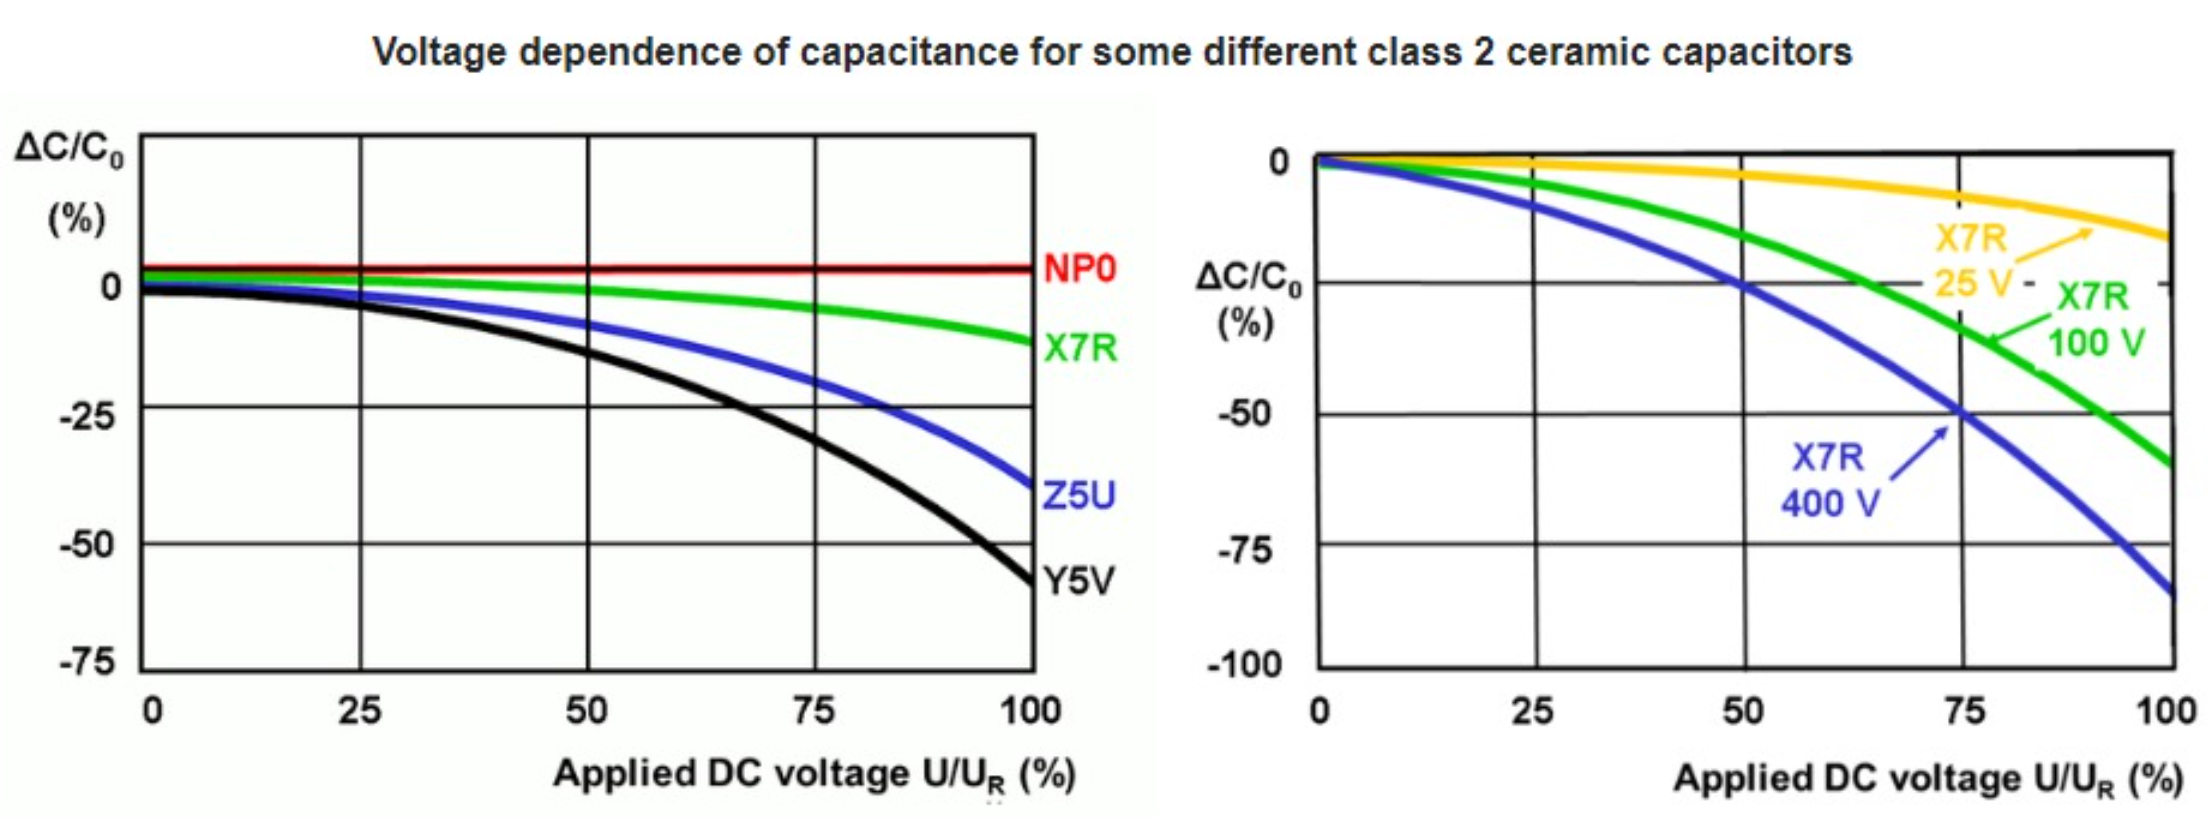
\includegraphics[width=0.8\textwidth]{napiecia_c.png}
    \caption{Spadek pojemności kondensatora ceramicznego wraz ze wzrostem napięcia}
\end{figure}

Wybrany kondensator jest klasy 2, wykonany z materiału X7R, co oznacza, że jego pojemność spadnie w przybliżeniu o 30\% dla napięcia 220\si{\volt}.
Zdecydowano się na zastosowanie 2 kondensatorów o wartości 2.2\si{\micro\farad} połączonych równolegle w celu zminimalizowania tętnień napięcia wyjściowego.
Ostatecznie pojemność oszacowana na:
\begin{equation}
    C_{220} = 2 \cdot (1-0.3) \cdot 2.2\si{\micro\farad} = 3.08\si{\micro\farad}
\end{equation}

Obliczono tętnienia dla dobranych wartości kondensatorów:
\begin{equation}
    \Delta V_{220} = \frac{V_{out}}{2 \cdot \frac{V_{out}}{I_{out}} \cdot C} \cdot \frac{D}{f_{sw}} = \frac{220}{2 \cdot \frac{220}{0.02} \cdot 3.08\si{\micro\farad}} \cdot \frac{0.945}{500000} \approx 6.1\si{\milli\volt}
\end{equation}

\begin{equation}
    \Delta V_{130} = \frac{V_{out}}{2 \cdot \frac{V_{out}}{I_{out}} \cdot C} \cdot \frac{D}{f_{sw}} = \frac{130}{2 \cdot \frac{130}{0.02} \cdot 3.08\si{\micro\farad}} \cdot \frac{0.908}{500000} \approx 5.89\si{\milli\volt}
\end{equation}

Wartości tętnień jest mniejsza niż założone 0.1\si{\volt}, co oznacza, że dobrano odpowiednie wartości kondensatorów.

\subsubsection{Dobór diody}
Oszacowano prąd diody na podstawie wzoru z noty katalogowej:
\begin{equation}
    I_{d} = \frac{I_{out}}{1-D} + \Delta I_{out} = \frac{0.02}{1-0.945} + 0.006 \approx 0.37\si{\ampere}
\end{equation}

Dioda powina mieć prąd przewodzenia większy niż 0.4\si{\ampere} oraz być szybką diodą shottky'ego, by zminimalizować straty w układzie.

Zdecydowano się na zastosowanie diody ES1G firmy Onsemi, 
która jest diodą super szybką, o prądzie przewodzenia 1\si{\ampere}, co jest wystarczające dla tego zastosowania.
Dioda ta ma maksymalne napięcie wsteczne 400\si{\volt}, co jest wystarczające.

\subsubsection{Dobór tranzystora}
Można założyć że prąd tranzystora to prąd cewki, czyli 0.468\si{\ampere}.
Zgodnie z noty katalogowej tranzystor powinien mieć następujące parametry:
\begin{itemize}
    \item Napięcie minimalnie drain-source: 250\si{\volt}
    \item Jak najmniejszy $R_{DS(on)}$
    \item Prąd przewodzenia większy niż 0.5\si{\ampere}
    \item Niskie napięcie progowe $V_{TH}$
    \item Jak najmniejszy ładunek bramki
    \item Wymaganego prąd bramki mniejszego niż 1\si{\ampere}
\end{itemize}
\newpage
Zdecydowano się na zastosowanie tranzystora N-Channel
MOSFET TPH5200FNH firmy Toshiba, który ma następujące parametry:
\begin{itemize}
    \item Napięcie drain-source: 250\si{\volt}
    \item $R_{DS(on)}$: 44\si{\milli\ohm}
    \item Prąd przewodzenia: 26\si{\ampere}
    \item Napięcie progowe: 2\si{\volt}
    \item Ładunek bramki: 22\si{\nano\coulomb}
    \item Rozpraszana moc: 2.5\si{\watt}
\end{itemize}

Prąd potrzebny na załączenie tranzystora można obliczyć na podstawie wzoru:
\begin{equation}
    I_{g} = Q_{g} \cdot f_{sw} = 22\si{\nano\coulomb} \cdot 500000 = 11\si{\milli\ampere}
\end{equation}


Tranzystor ten spełnia wszystkie założenia, a także ma bardzo niskie $R_{DS(on)}$, co pozwala na zminimalizowanie strat w układzie.

Moc wydzielana na tranzystorze można obliczyć na podstawie wzoru:

\begin{equation}
    P_{mos} = I_{l}^2 \cdot R_{DS(on)} = 0.468^2 \cdot 0.044 \approx 0.01\si{\watt}
\end{equation}

Moc jest bardzo niska, co oznacza, że tranzystor nie będzie się nagrzewał, a także nie będzie wymagał radiatora.

\subsubsection{Ustawienie napięcia wyjściowego}
Napięcie wyjściowe będzie regulowane, dlatego zdecydowano się na zastosowanie potencjometru cyfrowego włączonego w obwód sprzężenia zwrotnego.
Potencjometr cyfrowy będzie się komunikował z mikrokontrolerem za pomocą magistrali I2C, co pozwoli na zdalne ustawianie napięcia wyjściowego,
by regulować jasność lamp.

Wybrano potencjometr cyfrowy MCP4018T-103E/LT firmy Microchip,
który ma 128 poziomów ustawień, co pozwala na dokładne ustawienie napięcia wyjściowego,
wybrano wartość 10k\si{\ohm}, co pozwala na uzyskanie odpowiedniego zakresu ustawień napięcia wyjściowego.

Zgodnie z notą katalogową napięcie na pinie FB powinno wynosić 1.26\si{\volt}, napięcie to oznacza, że napięcie wyjściowe jest odpowiednie. 
Po przetestowaniu kilku kombinacji zdecydowano się na zastosowanie następujących rezystorów:
\begin{itemize}
    \item $R_{fb1} = 2.49\si{\mega\ohm}$
    \item $R_{fb2} = 14.39\si{\kilo\ohm}$
\end{itemize}

Obliczone napięcie na wyjściu dla potencjometru z nastawą 10\si{\kilo\ohm}:
\begin{equation}
    V_{out} = 1.26 \cdot (1 + \frac{R_{fb1}}{R_{fb2} + R_{pot}}) = 1.26 \cdot (1 + \frac{2.49\si{\mega\ohm}}{14.39\si{\kilo\ohm} + 10\si{\kilo\ohm}}) \approx 130.4\si{\volt}
\end{equation}
Obliczone napięcie na wyjściu dla potencjometru z nastawą 0\si{\ohm}:
\begin{equation}
    V_{out} = 1.26 \cdot (1 + \frac{R_{fb1}}{R_{fb2} + R_{pot}}) = 1.26 \cdot (1 + \frac{2.49\si{\mega\ohm}}{14.39\si{\kilo\ohm}}) \approx 220.6\si{\volt}
\end{equation}

Uzyskano zakres napięcia wyjściowego od 130.4\si{\volt} do 220.6\si{\volt}, co jest zgodne z założeniami projektowymi.

\subsubsection{Dobór rezystora ograniczającego prąd}
Układ ma możliwość ustawienia limitu prądu jaki będzie płynąć przez tranzystor,
co jest dodatkowym zabezpieczeniem przed uszkodzeniem tranzystora.

Najpierw obliczono wartość limitu szczytowego prądu przełączania zgodnie z notą katalogową:
\begin{equation}
    ISW_{limit} = \left(\frac{I_{out}}{1-D}+\frac{D \cdot V_{in}}{2 \cdot f_{sw} \cdot L}\right) = \left(\frac{0.02}{1-0.945}+\frac{0.945 \cdot 12}{2 \cdot 500000 \cdot 180\si{\micro\henry}}\right) \approx 0.426\si{\ampere}
\end{equation}

Następnie obliczono wartość rezystora ograniczającego prąd zgodnie z notą katalogową:
\begin{equation}
    R_{sense} = \frac{V_{SENSE} - (D \cdot V_{SENSE} \cdot V_{SL-ratio})}{ISW_{limit}} = \frac{156\si{\milli\volt} - (0.945 \cdot 156\si{\milli\volt} \cdot 0.49)}{0.426} \approx 74\si{\milli\ohm}
\end{equation}

Następnie sprawdzono warunek na maksymalną wartość rezystora ograniczającego prąd:
\begin{equation}
    R_{sense} < \frac{2 \cdot V_{SL} \cdot f_{sw} \cdot L}{V_{out} - (2 \cdot V_{IN})} = \frac{2 \cdot 92\si{\milli\volt} \cdot 500000 \cdot 180\si{\micro\henry}}{220 - (2 \cdot 12)} \approx 84\si{\milli\ohm}
\end{equation}

Zdecydowano się na zastosowanie rezystora o wartości 75\si{\milli\ohm}, który spełnia wszystkie założenia.
Został również dodany kondensator o wartości 10\si{\pico\farad} w celu zminimalizowania tętnień napięcia na rezystorze,
oraz rezystor kompensujący 100\si{\ohm}.
\subsubsection{Schemat}
\begin{figure}[H]
    \centering
    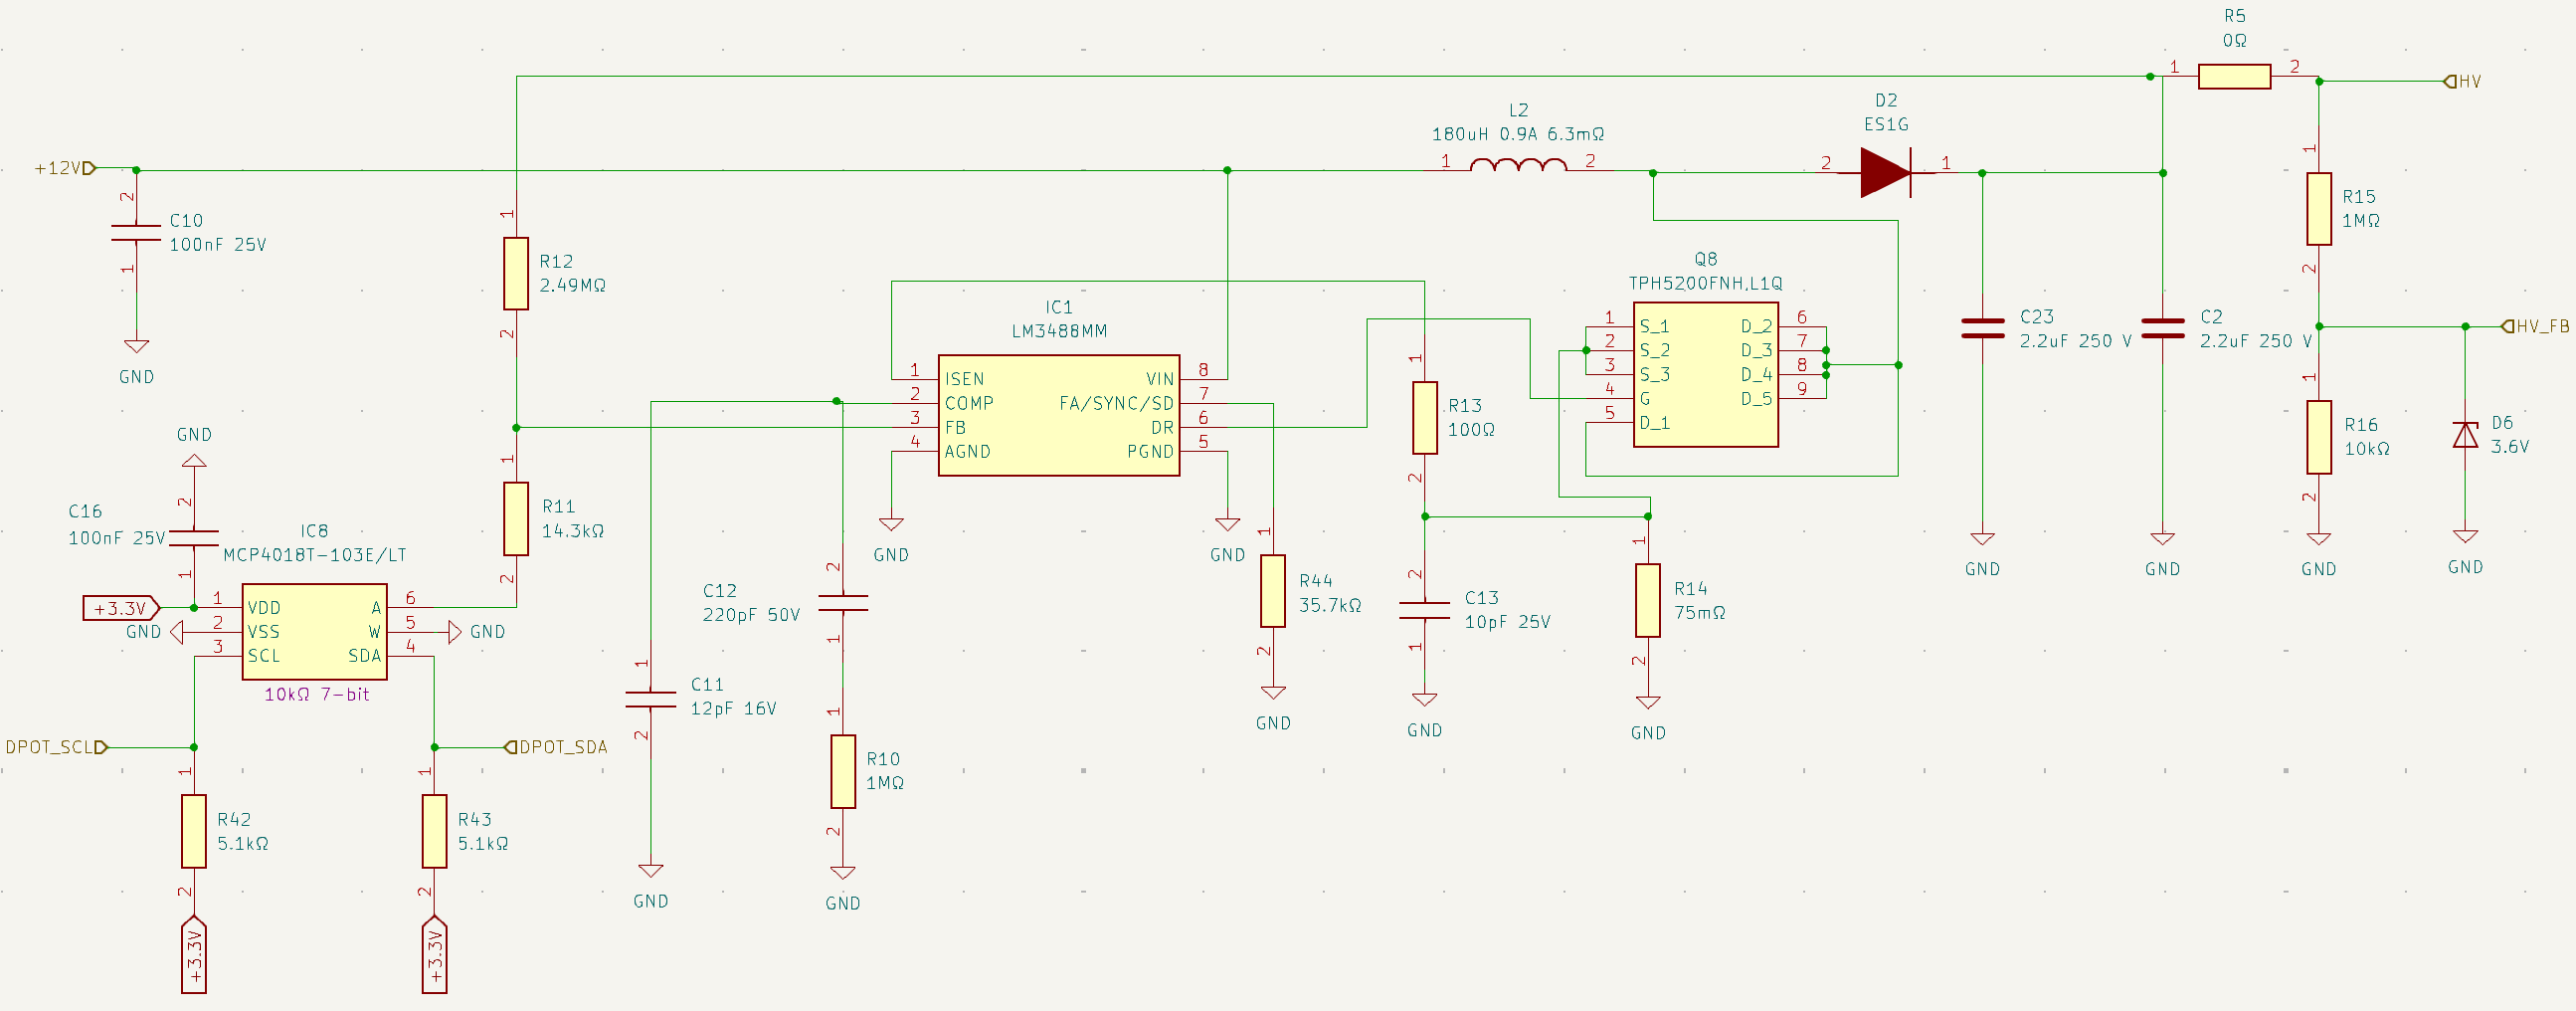
\includegraphics[width=1.1\textwidth]{schemat.png}
    \caption{Schemat przetwornicy 12V na HV}
\end{figure}
\end{document}
